\documentclass[a4paper,11pt]{amsart}
\usepackage[T1]{fontenc}
\usepackage{amsmath}
\usepackage{amssymb}
\usepackage{enumitem}
\usepackage{graphicx}
\usepackage{tikz}
\author{Piotr Sl 1693...}
\address{UWM w Olsztynie}
\email{sl...@wp.pl }
\title{Przykładowy kolokwium wariant 0}
\renewcommand{\contentsname}{Spis treści}
\renewcommand{\figurename}{Rysunek}
\begin{document}
\maketitle
\tableofcontents
\section{Tekst}
Tutaj testujemy czcionki. To jest tekst normalny, 12pt. \textbf{Lorem ip-
sum dolor sit amet, consectetur adipiscing elit, sed do eiusmod
tempor incididunt ut labore et dolore magna aliqua.} 
\textit{Ut enim ad
minim veniam, quis nostrud exercitation ullamco laboris nisi ut aliquip
ex ea commodo consequat.} 
\begin{Huge}Duis aute irure dolor in
reprehenderit in voluptate velit esse
cillum dolore eu fugiat nulla pariatur.
\end{Huge}
\section{Wzory}
\emph{Szereg harmoniczny} to szereg liczbowy postaci
\begin{equation}
\displaystyle\sum^\infty_{n=1}\frac{1}{n}=1+\frac{1}{2}+\frac{1}{3}+...
\end{equation}
Kolejny sumy częściowe 
$H_N=\displaystyle\sum^N_{n=1}\frac{1}{n}, N \in \mathbb{N}$ 
szeregu (1) nazywają się \emph{liczbami harmonicznymi}. 
Dla liczb harmonicznych spełnia się
$$H_N\approx \textrm{ln}  n + \gamma,$$
gdzie ln jest logarytmem naturalnym, a $y \approx 0.577$ jest konstantą
\textbf{Eulera-Masheroni}.  \newpage
Nazwa szeregu pochodzi stąd, że każdy wyraz szeregu dla $k\geq 2$ jest \textbf{średnią harmoniczną} dwóch wyrazów bezpośrednio z nim sąsiadujących:
$$II(\frac{1}{n-1},\frac{1}{n+1})=\frac{1+1}{(\frac{1}{n-1})^{-1}+(\frac{1}{n+1})^{-1}}=\frac{2}{(\frac{1}{n-1})^{-1}+(\frac{1}{n+1})^{-1}}
=\frac{2}{(n-1)+(n+1)}=\frac{1}{n}.$$
\section{Macierze}
\emph{Macierz stochastyczna} - macierz kwadratowa, której elementami 
są nieujemne liczby rzeczywiste i w której sumy elementów
dają 1. W zależnoDci od tego czy sumy elementów w każdym wierszu
czy w każdej kolumnie dają 1, macierz stochastyczną nazywamy odpo-
wiednio prawą lub lewą macierzą stochastyczną. Jeśli macierz jest lewą
i prawą macierzą stochastyczną, to nazywa się ją macierzą podwójnie
stochastyczną. Macierz
$$P=
\begin{bmatrix}
P_{1,1}&P_{1,2}&...&P_{1,j}&...&P_{1,\alpha}\\
P_{2,1}&P_{2,2}&...&P_{2,j}&...&P_{2,\alpha}\\
...\\
P_{i,1}&P_{i,2}&...&P_{i,j}&...&P_{i,\alpha}\\
...\\
P_{\alpha,1}&P_{\alpha,2}&...&P_{\alpha,j}&...&P_{\alpha,\alpha}
\end{bmatrix},$$
jest prawą stochastyczną, jeżeli $\sum^\alpha_{j=1}P_{i,j}=1$ dla każdego $i=\overline{1,\alpha}$ oraz \newline
lewą stochastyczną jeżeli $\sum^\alpha_{i=1}P_{i,j}=1$ dla każdego $j=\overline{1,\alpha}.$
\section{Spis}
\begin{enumerate}[label=\Alph*)]
\item ryby,
\begin{enumerate}[label=A.b.\alph*)]
\item śluzice (Myxini),
\item Petromyzontida,
\begin{enumerate}[label=A.b.\Roman*)]
\item Geotriidae
\item Mordaciidae
\item Petromyzontidae minogowate
\end{enumerate}
\item ryby chrzęstnoszkieletowe (Chondrichthyes),
\begin{enumerate}[label=A.b.\Roman*)]
\item spoduste (Elasmobranchii)
\begin{enumerate}[label=|\roman*|]
\item rekiny
\item płaszczki
\end{enumerate}
\item zrosłogłowe (Holocephali)
\end{enumerate}
\item ryby kostnoszkieletowe (Osteichthyes, w tym czworonogi)
\end{enumerate}
\item płazy,
\item gady,
\item ptaki,
\item ssaki.
\end{enumerate}
\newpage
\section{Obrazek}
Zgredek (ang. Dobby) - skrzat domowy oraz wieloletni służący w
dworze Malfoyów. W 1992 roku, z pomoc¡ Harry'ego Pottera, został
uwolniony z rąk Lucjusza Malfoya. Pomagał chłopcu, kiedy ten go
potrzebował i zawsze był wobec niego lojalny. Zginął z rak Bellatriks
Lestrange, która rzuciła w niego sztyletem, gdy teleportował się z Ronem, Harrym i Hermioną, podczas ucieczki z dworu Malfoyów.
\begin{figure}[htbp]
\includegraphics[scale=0.5]{dobby.jpg}
\caption{Zgredek}
\end{figure}
\section{Rysunek}
\begin{figure}[htbp]
\centering
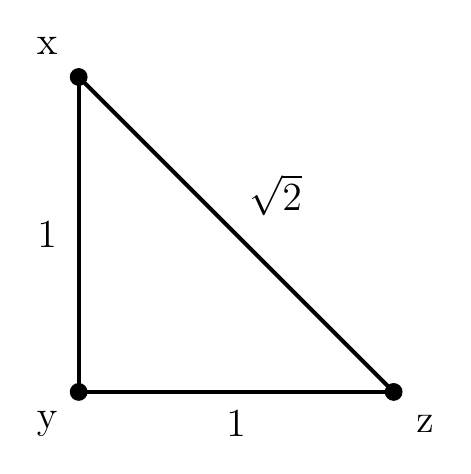
\begin{tikzpicture}
\draw[black, fill=black] (-2,2) circle (3px);
\draw[black, fill=black] (-2,-2) circle (3px);
\draw[black, fill=black] (2,-2) circle (3px);
\draw[line width=0.5mm, black](-2,2) to (-2,-2);
\draw[line width=0.5mm, black](-2,-2) to (2,-2);
\draw[line width=0.5mm, black](2,-2) to (-2,2);
\node at (-2.4,2.4) {\Large x};
\node at (-2.4,-2.4) {\Large y};
\node at (2.4,-2.4) {\Large z};
\node at (-2.4,0) {\Large 1};
\node at (0,-2.4) {\Large 1};
\node at (0.5,0.5) {\Large $\sqrt{2}$};
\end{tikzpicture}
\caption{Graf}
\end{figure}
\end{document}